\section{Odometry}\label{sec:visual-odometry}
As introduced in \S1.2, the problem of odometry is about the estimation of the change in a robot's pose over time.

The odometry, also known as self-localization, an be classified in different ways, in \S2.2.1 there is a more detailed description of the different types of odometry.

\subsection{Taxonomy}\label{subsec:tassonomy}
There different types of odometry, which based on the classification of ~\cite{vo_state_of_art} can be divided into two main categories: \textit{GNSS available} and \textit{GNSS not available}.
\begin{figure}[H]
    \centering
    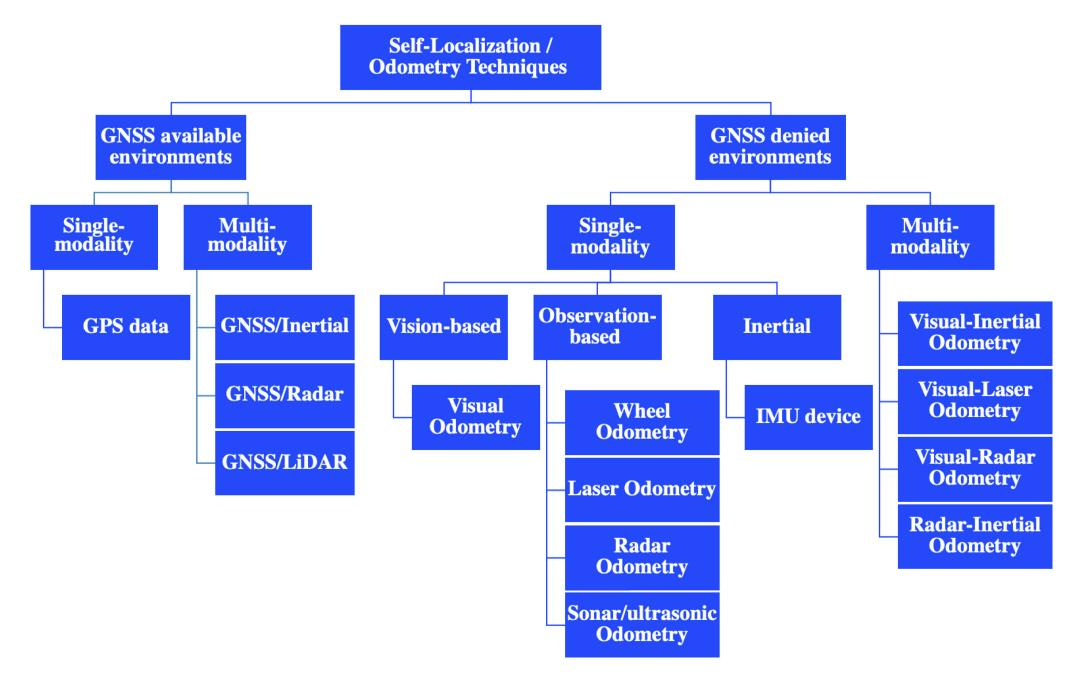
\includegraphics[width=\textwidth]{images/2_2_taxonomy_odometry}
    \caption{Taxonomy of odometry techniques}\label{fig:odometry-taxonomy}
\end{figure}

\subsection{Reference systems}\label{subsec:reference-systems}
To tackle the problem of odometry, we need as to choose the representation system to adopt.
There are many way of representing the pose of the camera or the robot, but the most common are the \textit{Euler angles} and the \textit{quaternions} and \textit{rotation matrix} combined with \textit{translation matrix}.
% TODO add how to translate the poses origin.
\subsection{State of the art}\label{subsec:state-of-the-art}
